% Als je labels toe wilt voegen, doe het dan consequent
% voor een section ---> \label{sec:name_of_block}
%voor een subsection ---> \label{ssec:name_of_subsec}
%voor een subsubsec --> \label{sssec:name_of_subsubsec} en zo door

%Template voor elk apart blok EPO3 A4
\documentclass{scrartcl} % scrartcl of scrreprt
% Include all project wide packages here.
\usepackage{fullpage}
\usepackage{polyglossia}
\setmainlanguage{dutch}
\usepackage{csquotes}
\usepackage{graphicx}
\usepackage{epstopdf}
\usepackage{pdfpages}
\usepackage{caption}
\usepackage[list=true]{subcaption}
\usepackage{float}
%\usepackage{mathtools}
\usepackage{standalone}
\usepackage{import}
\usepackage{tocloft}
\usepackage{wrapfig}
\usepackage{authblk}
\usepackage{array}
\usepackage{booktabs}
\usepackage[toc,page,title,titletoc]{appendix}
\usepackage{xunicode}
\usepackage{amsmath}
\usepackage{fontspec}
\usepackage{unicode-math}
\usepackage[
    backend=bibtexu,
	texencoding=utf8,
bibencoding=utf8,
    style=ieee,
    sortlocale=nl_NL,
    language=auto
]{biblatex}
\usepackage{listings}
\newcommand{\includecode}[3][c]{\lstinputlisting[caption=#2, escapechar=, style=#1]{#3}}
\newcommand{\superscript}[1]{\ensuremath{^{\textrm{#1}}}}
\newcommand{\subscript}[1]{\ensuremath{_{\textrm{#1}}}}


\newcommand{\chapternumber}{\thechapter}
\renewcommand{\appendixname}{Bijlage}
\renewcommand{\appendixtocname}{Bijlagen}
\renewcommand{\appendixpagename}{Bijlagen}

\usepackage[hidelinks]{hyperref} %<--------ALTIJD ALS LAATSTE
 
\renewcommand{\familydefault}{\sfdefault}

\setmainfont[Ligatures=TeX]{Myriad Pro}
\setmathfont{Asana Math}
\setmonofont{Lucida Console}

\usepackage{titlesec, blindtext, color}
\definecolor{gray75}{gray}{0.75}
\newcommand{\hsp}{\hspace{20pt}}
\titleformat{\chapter}[hang]{\Huge\bfseries}{\chapternumber\hsp\textcolor{gray75}{|}\hsp}{0pt}{\Huge\bfseries}
\renewcommand{\familydefault}{\sfdefault}
\renewcommand{\arraystretch}{1.2}
\setlength\parindent{0pt}

%For code listings
\definecolor{black}{rgb}{0,0,0}
\definecolor{browntags}{rgb}{0.65,0.1,0.1}
\definecolor{bluestrings}{rgb}{0,0,1}
\definecolor{graycomments}{rgb}{0.4,0.4,0.4}
\definecolor{redkeywords}{rgb}{1,0,0}
\definecolor{bluekeywords}{rgb}{0.13,0.13,0.8}
\definecolor{greencomments}{rgb}{0,0.5,0}
\definecolor{redstrings}{rgb}{0.9,0,0}
\definecolor{purpleidentifiers}{rgb}{0.01,0,0.01}


\lstdefinestyle{csharp}{
language=[Sharp]C,
showspaces=false,
showtabs=false,
breaklines=true,
showstringspaces=false,
breakatwhitespace=true,
escapeinside={(*@}{@*)},
columns=fullflexible,
commentstyle=\color{greencomments},
keywordstyle=\color{bluekeywords}\bfseries,
stringstyle=\color{redstrings},
identifierstyle=\color{purpleidentifiers},
basicstyle=\ttfamily\small}

\lstdefinestyle{c}{
language=C,
showspaces=false,
showtabs=false,
breaklines=true,
showstringspaces=false,
breakatwhitespace=true,
escapeinside={(*@}{@*)},
columns=fullflexible,
commentstyle=\color{greencomments},
keywordstyle=\color{bluekeywords}\bfseries,
stringstyle=\color{bluestrings},
identifierstyle=\color{purpleidentifiers}
}

\lstdefinestyle{vhdl}{
language=VHDL,
showspaces=false,
showtabs=false,
breaklines=true,
showstringspaces=false,
breakatwhitespace=true,
escapeinside={(*@}{@*)},
columns=fullflexible,
commentstyle=\color{greencomments},
keywordstyle=\color{bluekeywords}\bfseries,
stringstyle=\color{redstrings},
identifierstyle=\color{purpleidentifiers}
}

\lstdefinestyle{xaml}{
language=XML,
showspaces=false,
showtabs=false,
breaklines=true,
showstringspaces=false,
breakatwhitespace=true,
escapeinside={(*@}{@*)},
columns=fullflexible,
commentstyle=\color{greencomments},
keywordstyle=\color{redkeywords},
stringstyle=\color{bluestrings},
tagstyle=\color{browntags},
morestring=[b]",
  morecomment=[s]{<?}{?>},
  morekeywords={xmlns,version,typex:AsyncRecords,x:Arguments,x:Boolean,x:Byte,x:Char,x:Class,x:ClassAttributes,x:ClassModifier,x:Code,x:ConnectionId,x:Decimal,x:Double,x:FactoryMethod,x:FieldModifier,x:Int16,x:Int32,x:Int64,x:Key,x:Members,x:Name,x:Object,x:Property,x:Shared,x:Single,x:String,x:Subclass,x:SynchronousMode,x:TimeSpan,x:TypeArguments,x:Uid,x:Uri,x:XData,Grid.Column,Grid.ColumnSpan,Click,ClipToBounds,Content,DropDownOpened,FontSize,Foreground,Header,Height,HorizontalAlignment,HorizontalContentAlignment,IsCancel,IsDefault,IsEnabled,IsSelected,Margin,MinHeight,MinWidth,Padding,SnapsToDevicePixels,Target,TextWrapping,Title,VerticalAlignment,VerticalContentAlignment,Width,WindowStartupLocation,Binding,Mode,OneWay,xmlns:x}
}

%defaults
\lstset{
basicstyle=\ttfamily\small,
extendedchars=false,
numbers=left,
numberstyle=\ttfamily\tiny,
stepnumber=1,
tabsize=4,
numbersep=5pt
}


\author{}% <------fill in your name
\title{EPO3: Eindrapport - Draw-pixel}

\begin{document}
\section{Drawpixel} %<----- fill in section name
\label{sec:drawpixel} % <-----fill in lable name

% describe function of block
Drawpixel is het blok dat het tekenen van een pixel implementeerd. Drawpixel ontvangt via de instructiedecoder std\_standard\_logic vectoren x , y en color van de CPU. In de specificaties wordt ingegaan  op de lengte van deze vectoren. In het gedeelte daaronder wordt de verdere implementatie en het testen beschreven.

%specificaties blok (copy paste)
\subsection{Specificaties}
\label{ssec:specs_dp}
Door deze module worden aparte pixels getekend, hiervoor zijn de x- en y-coördinaten en de kleur van de pixel nodig. Drawpixel dient asb, y en x in een vector te plaatsen van lengte SizeRAMAddr, gedefinieerd in de package file. X en y zijn ook vectoren met lengten gedefinieerd in de package. Ook dient de color vector naar ramdata geschreven te worden.  Er moet alleen bij enable \& draw\_can\_access = hoog naar RAM geschreven worden, waarbij draw\_write gedurende het schrijven hoog is. (voor de controller)  Nadat er geschreven is, moet done gedurende een klokslag hoog worden. Er mag alleen in het niet actieve RAM geschreven worden, dus wanneer asb '0' is. 

\begin{table}[H]
\centering
\caption{Specificaties van de Pixel Draw Module}
\label{tab:spec-pixel-draw}
\begin{tabular}{c c c}
	\hline\hline
 	Naam & Modus & Type\\
 	\hline	
	clk & in & std\_logic \\
	reset & in & std\_logic \\
	enable& in & std\_logic \\
	color & in & std\_logic\_vector(SizeColor-1 downto 0) \\
	x & in & std\_logic\_vector(SizeX-1 downto 0) \\
	y & in & std\_logic\_vector(SizeY-1 downto 0) \\
	asb & in & std\_logic \\
	done & out & std\_logic \\
	ramaddr &out & std\_logic\_vector(SizeRAMAddr-1 downto 0) \\
	ramdata &out & std\_logic\_vector(SizeRAMData-1 downto 0) \\
	draw\_write &out & std\_logic \\
	draw\_can\_access & in & std\_logic \\
  	\hline
\end{tabular}
\end{table}


%VHDL
\subsection{VHDL}
\label{ssec:vhdl_dp}
\subsubsection{Entity}
De entity is opgebouwd volgens de specificaties in tabel \ref{tab:spec-pixel-draw}. De in- en uitgangen zijn letterlijk overgenomen en zijn schaalbaar, zoals te zien in de tabel. 

\subsubsection{Behaviour}
De behaviour is opgedeeld in een sequentieel gedeelte waar de state 'busy' wordt opgeslagen en een combinatorisch gedeelte waar de signalen oe, draw\_write, done en de state worden bepaald. Oe is een tussensignaal op basis waarvan bepaald wordt of ramaddr en ramdata geschreven worden. Het is belangrijk dat de uitgangen 'Z' worden indien oe = 1 niet klopt, omdat de draad waarop de uitgang gezet wordt een bidirectional bus is. Het sequentiele process wordt getriggered op de clk, het combinatorische process op een verandering in reset, enable, draw\_can\_access of busy. 

%Testplan VHDL
\subsection{Testplan}
De eerste test betreft het simuleren van de behaviour met een testbench. Dit betreft een lege entity en een behaviour waarin een x-vector, y-vector en color-vector aangeboden worden volgens de lengte in de package file. Er is gekozen om de modelsim-simulatie eenmalig per blok op te nemen. 
\begin{figure} [h!]
\centering
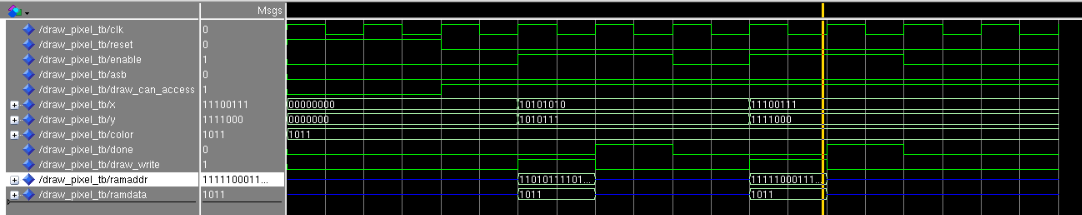
\includegraphics [scale = 0.8] {resource/dp_sim}
\caption{Modelsim simulatie behavioural of drawpixel}
\label{fig:dp_sim}
\end{figure}

%Synthese
\subsection{Synthese}
In figuur \ref{fig:dpcircuit} hierboven zijn duidelijk alle tri-state buffers te zien, zonder de flipflops erachter. Uiteindelijk is het circuit netjes gerout met een efficientie van 67,83\% en slechts 516 transistors. In overleg met Erwin is besloten het circuit deze vorm te geven. Drawpixel is namelijk een klein blok en goed te passen naast de grotere vierkante blokken op de chip in deze vorm. Dit zorgt wel voor meer transistoren, eerst was een efficientie van 85\% procent mogelijk. 


%Switchlevel test
\subsection{Switchlevel}
Op switchlevel niveau wordt de simulatie op transistor niveau vergeleken met de simulatie op vhdl niveau. Hierbij wordt er vanuit de list-file een command file gemaakt. Vervolgens wordt via layout\simulate en show\_result een simulatie geopend. Nu kan figuur \ref{fig:dp_sim} hiermee op het oog vergeleken worden. De optie compare geeft de mogelijkheid om dit exact te doen met GoWithTheFlow. De ref-file van de simulatie in figuur \ref{fig:dp_sim} wordt dan vergeleken met de res-file van de switch level simulatie. Is de implementatie goed dan horen alle waardes overeen te komen, op de eerste na. In ons ontwerp bevinden zich echter 'Z'-uitgangen, die door de compare niet goed begrepen worden. De noodzaak van 'Z's is al toegelicht. 


\begin{figure} [h!]
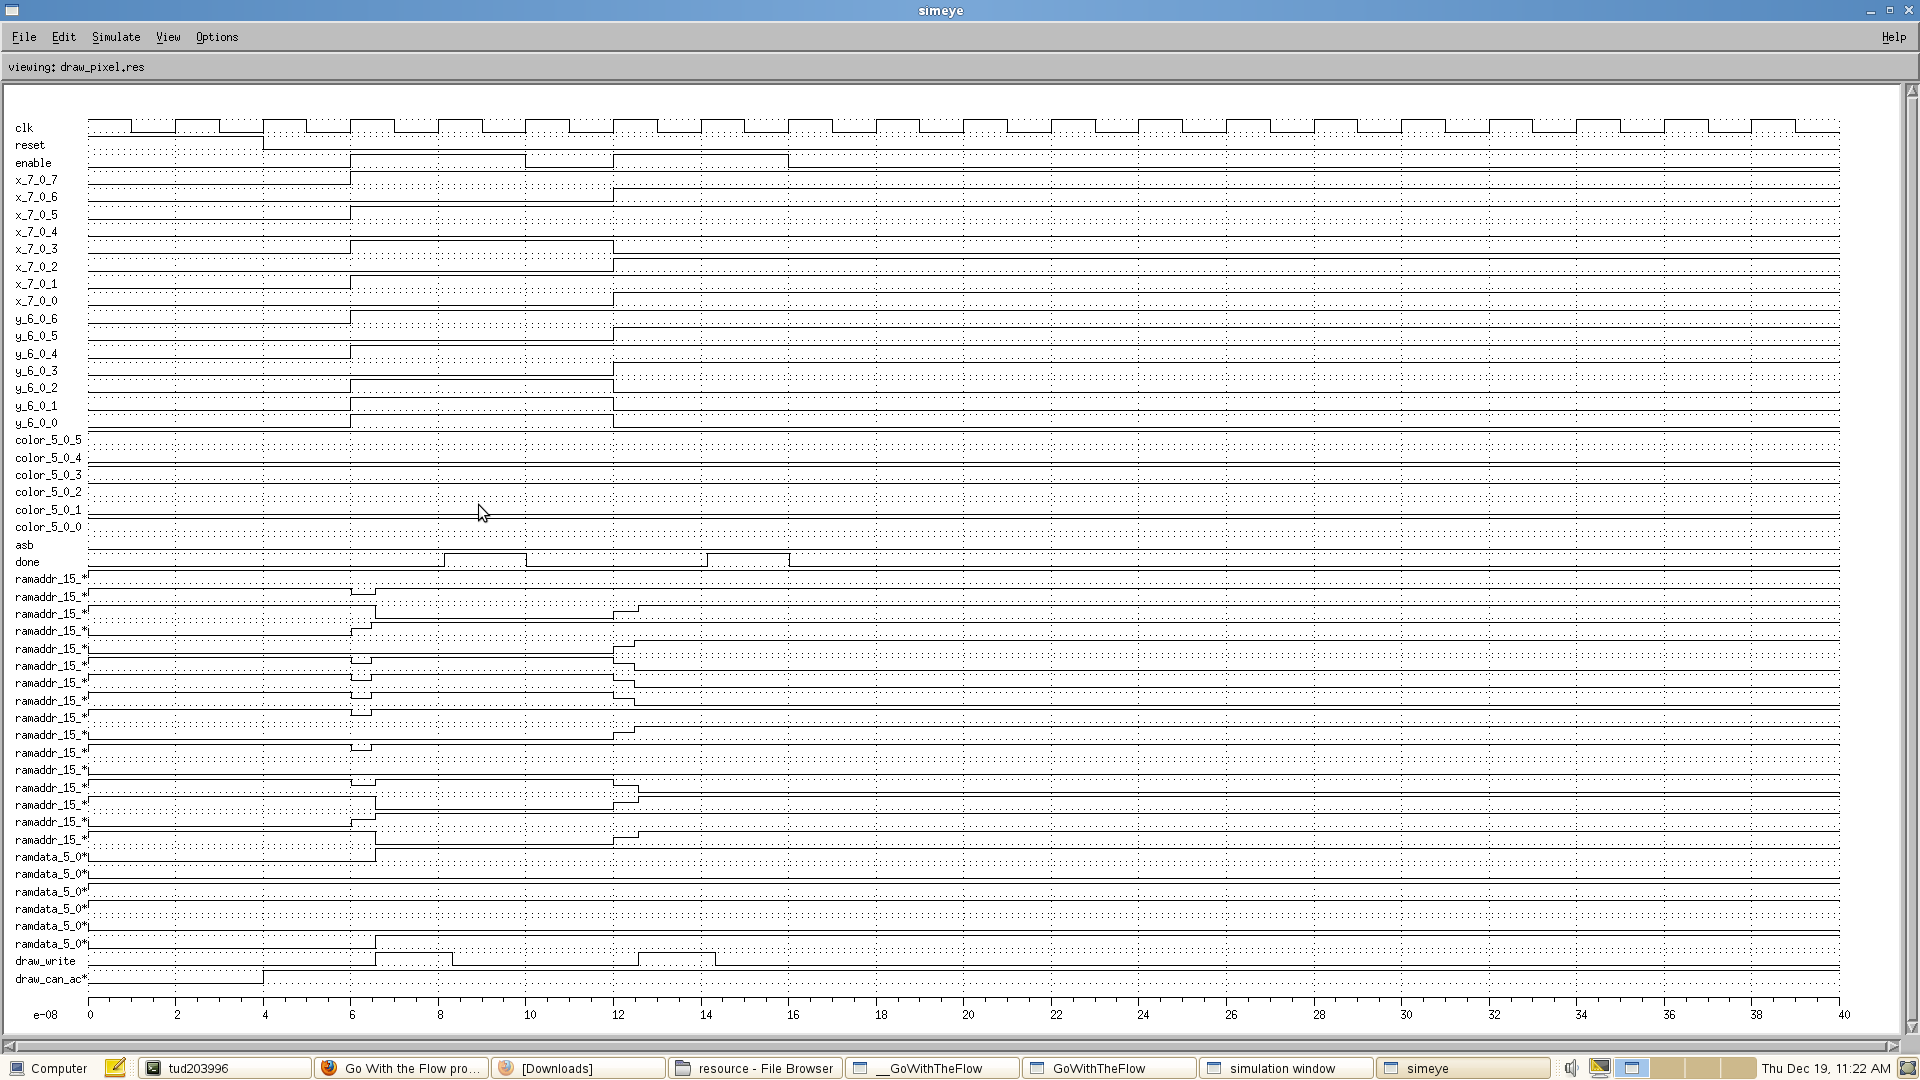
\includegraphics [width = \textwidth] {resource/dp_sw_lev}
\caption{Simulatie op transistor niveau}
\label{fig:dp_sw_lev}
\end{figure}



\begin{figure} [h!]
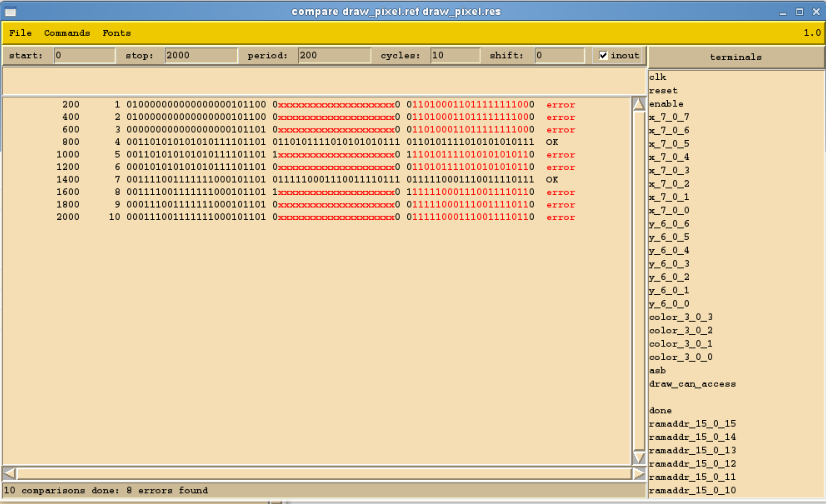
\includegraphics [width = \textwidth] {resource/dp_comp}
\caption{GWTF compare}
\label{fig:dp_comp}
\end{figure}






%Extracted test
\subsection{Extracted}
Om 


%Conclusie
\subsection{Conclusie}
Nadat de VHDL code als werkend kon worden beschouwd, moest de code worden gesynthetiseerd. In eerste instantie leverde dat 3000 transistoren op. Er is toen besloten de VHDL code op te delen in een sequentieel en een combinatorisch deel. Daarna is de code opnieuw gesynthetiseerd.  Echter na deze synthetisatie en ook wanneer er zelf blokken werden versleept kwamen we uit op 1500 transistors. Het grotere probleem was het feit dat hij hem moeilijk kon routen, maar na het circuit nader te bekijken zagen we dat er onnodig flipflops na da tri-state buffer kwamen, die vervolgens ook geen ‘Z’ konden opslaan. Dit zorgde voor de nodige errors, en een onnodig gebruik van extra flipflops. In de VHDL code hebben we vervolgens alle onnodige flipflops eruit gewerkt, waardoor alles in een keer werkte, en we dus ons uiteindelijke resultaat hebben behaald met slechts 516 transistors in plaats van 3000. 






\end{document}
